\chapter{Resultados}


% TODO: Falar pq usa os dados compartilhados. Divisão por cidade. Durante tela de busca de produtos, vincular com a seção de armazenamento/dados compartilhados.

\iffalse
Exemplo de citação longa:

\begin{citacao}
\lipsum[1] \cite[5.3]{abntex2cite-alf}
\end{citacao}

Exemplo de citação curta:

Segundo \cite{abntex2cite}, "Lorem ipsum dolor sit amet, consectetur adipiscing elit. Suspendisse adipiscing eu libero non ultricies. Donec accumsan, turpis ut malesuada facilisis, felis augue porta quam, et lacinia turpis ligula et risus.".

Conter imagens da interface do aplicativo, isto é, das telas;
Como o usuário acessa os dados presentes no App;
Discutir sobre os prós e contras do desenvolvimento;
Limitações do App e suas tecnologias utilizadas;
O banco de dados centralizado:
Discutir sobre o BD no celular do usuário vs um BD central;
Trabalhos futuros:
Registros do usuário;
Monitorar para diferentes mercados, produtos e cidades;
Desvantagens da tecnologia utilizada pelo BD:
Comparar os tipos de BDs: relacionais e não-relacionais;
\fi

\section{O Aplicativo Desenvolvido}

Conforme apresentado na seção \ref{desenvApp}, o aplicativo foi desenvolvido utilizando o React Native e tendo utilizado alguns pacotes de estilização. O aplicativo é funcional, ou seja, é possível efetuar a instalação do mesmo em um smartphone e utilizar todos os seus recursos, no entanto, o mesmo não se encontra disponível para download através das lojas de aplicativos AppStore e PlayStore, respectivamente dos sistemas iOS e Android.

Embora não seja possível instalar a aplicação através das lojas oficiais das plataformas, para o sistema Android é possível efetuar a instalação de aplicativos por outros meios. \textbf{\textcolor{red}{[FALAR UM POUCO MAIS]}}

\subsection{Apresentação do Aplicativo}

% FIXME: Ajustar a imagem
% FIXME: Adicionar referencia a imagem
\begin{figure}[h]
    \centering
    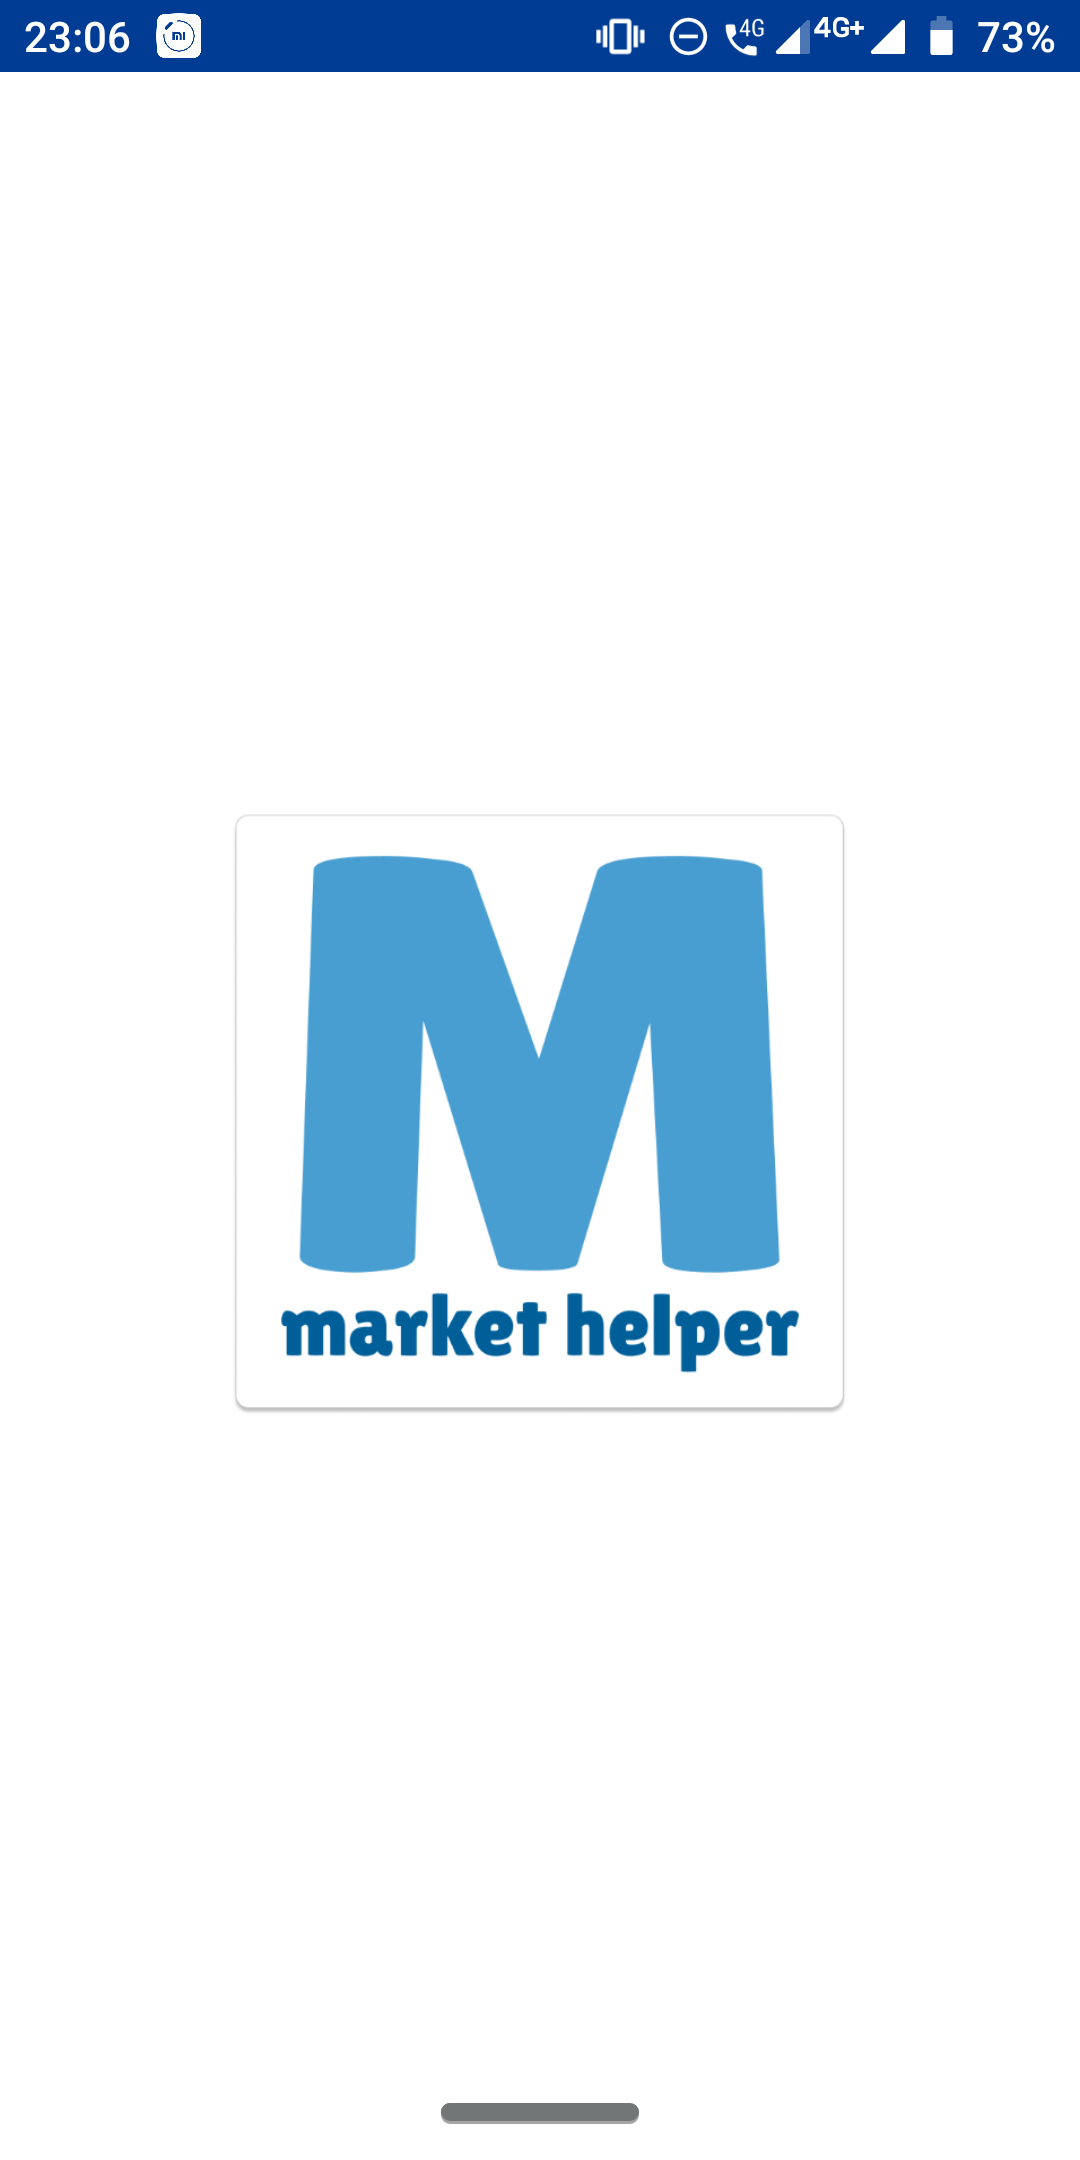
\includegraphics[scale=0.15]{tcc/figures/app/app_loading.png}
    \caption{Tela de carregamento inicial}
    \label{appLoadingFig}
\end{figure}

A figura \ref{appLoadingFig} representa a primeira tela que o usuário obtém ao efetuar a abertura da aplicação, além disso, essa tela é mostrada para que os recursos mínimos necessários ao aplicativo possam ser carregados. Com isso, sempre que o app for inicializado mostrará essa tela. Caso o usuário saia e vá para outro aplicativo, essa tela não será mostrada pois os recursos ainda estão em memória, mas caso o usuário encerre a aplicação, na próxima vez que houver a abertura, será necessário novamente efetuar o carregamento, logo, a tela de carregamento inicial será novamente exibida.

% FIXME: Ajustar a imagem
% FIXME: Adicionar referencia a imagem
\begin{figure}[h]
    \centering
    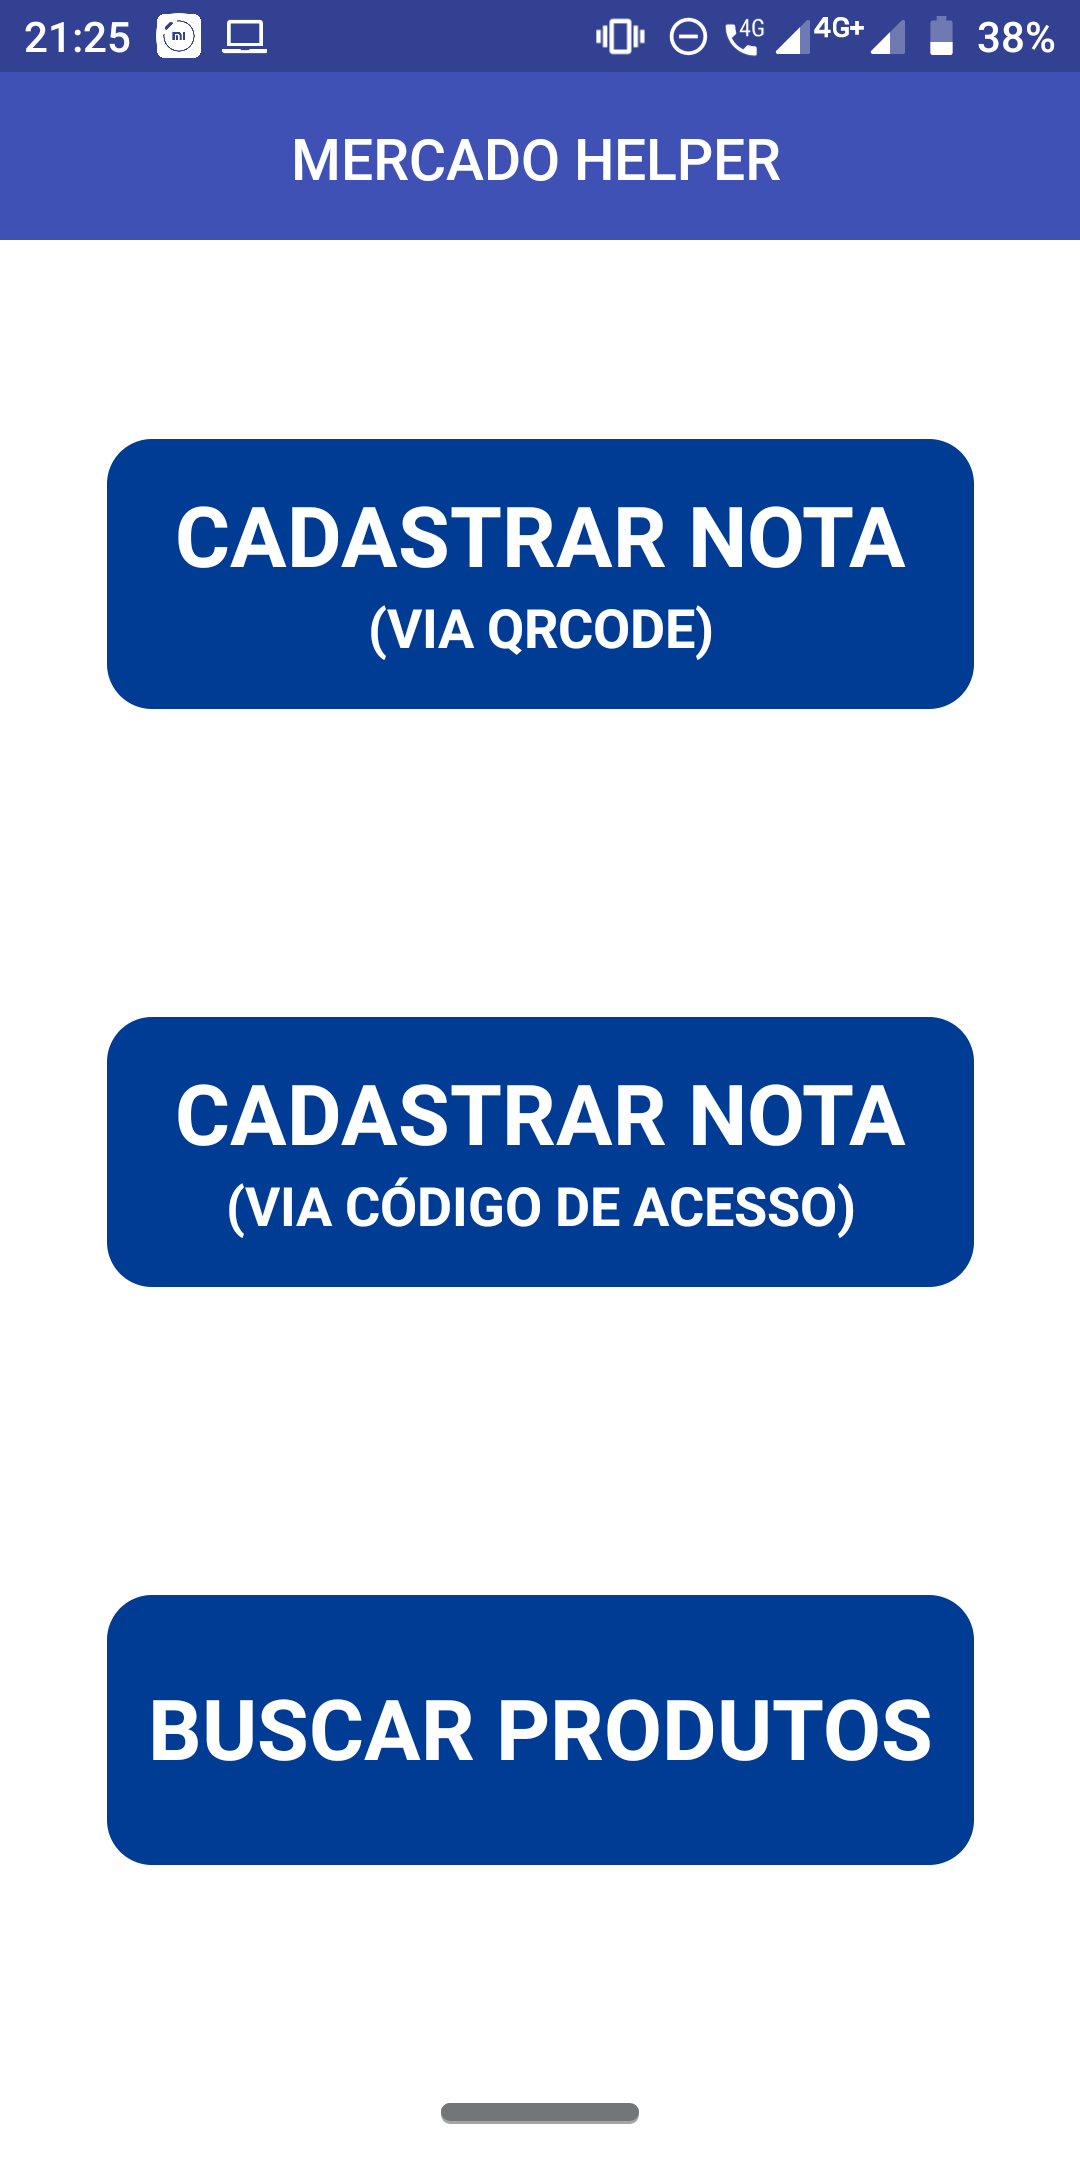
\includegraphics[scale=0.15]{tcc/figures/app/app_home.png}
    \caption{Tela principal}
    \label{appHomeFig}
\end{figure}

Após o carregamento desses recursos, o usuário é automaticamente redirecionado para a tela principal do aplicativo, que é demonstrada através da figura \ref{appHomeFig}. A partir dessa tela, é possível efetuar a adição das notas fiscais como a busca por produto através dos atalhos.

No primeiro botão, é possível efetuar a adição da NFC-e através do QRCode presente na mesma. Para tal funcionalidade, é necessário que o dispositivo possua uma câmera e que o usuário conceda permissão para uso da mesma.

No segundo botão, o usuário poderá efetuar a adição através do código de acesso e no último botão, o mesmo poderá consultar a base de dados para obter as informações referentes aos produtos.

\subsection{Adição das Notas Fiscais}

O usuário poderá efetuar a adição das notas através de duas formas, a primeira que é através do QRCode presente nas versões impressa das mesmas bem como através do código de acesso também disponível na versão física da nota.

Dependendo da forma de adição desejada pelo usuário, o mesmo será redirecionado para outras telas que serão apresentadas logo abaixo.

O meio mais rápido de adicionar é aquele que utiliza o QRCode, pois basta apontar a câmera no smartphone para o código que a leitura do mesmo será feita instantaneamente.

Caso ocorra problemas na leitura desse código, o usuário poderá tentar adicionar através do código de acesso. Esse meio é um pouco mais lento, pois além de inserir esse código de 44 dígitos, será necessário adicionar um código de verificação da solicitação, isto é, o código captcha.

\subsubsection{Através do QRCode}

% FIXME: Ajustar a imagem
% FIXME: Adicionar referencia a imagem
\begin{figure}[h]
    \centering
    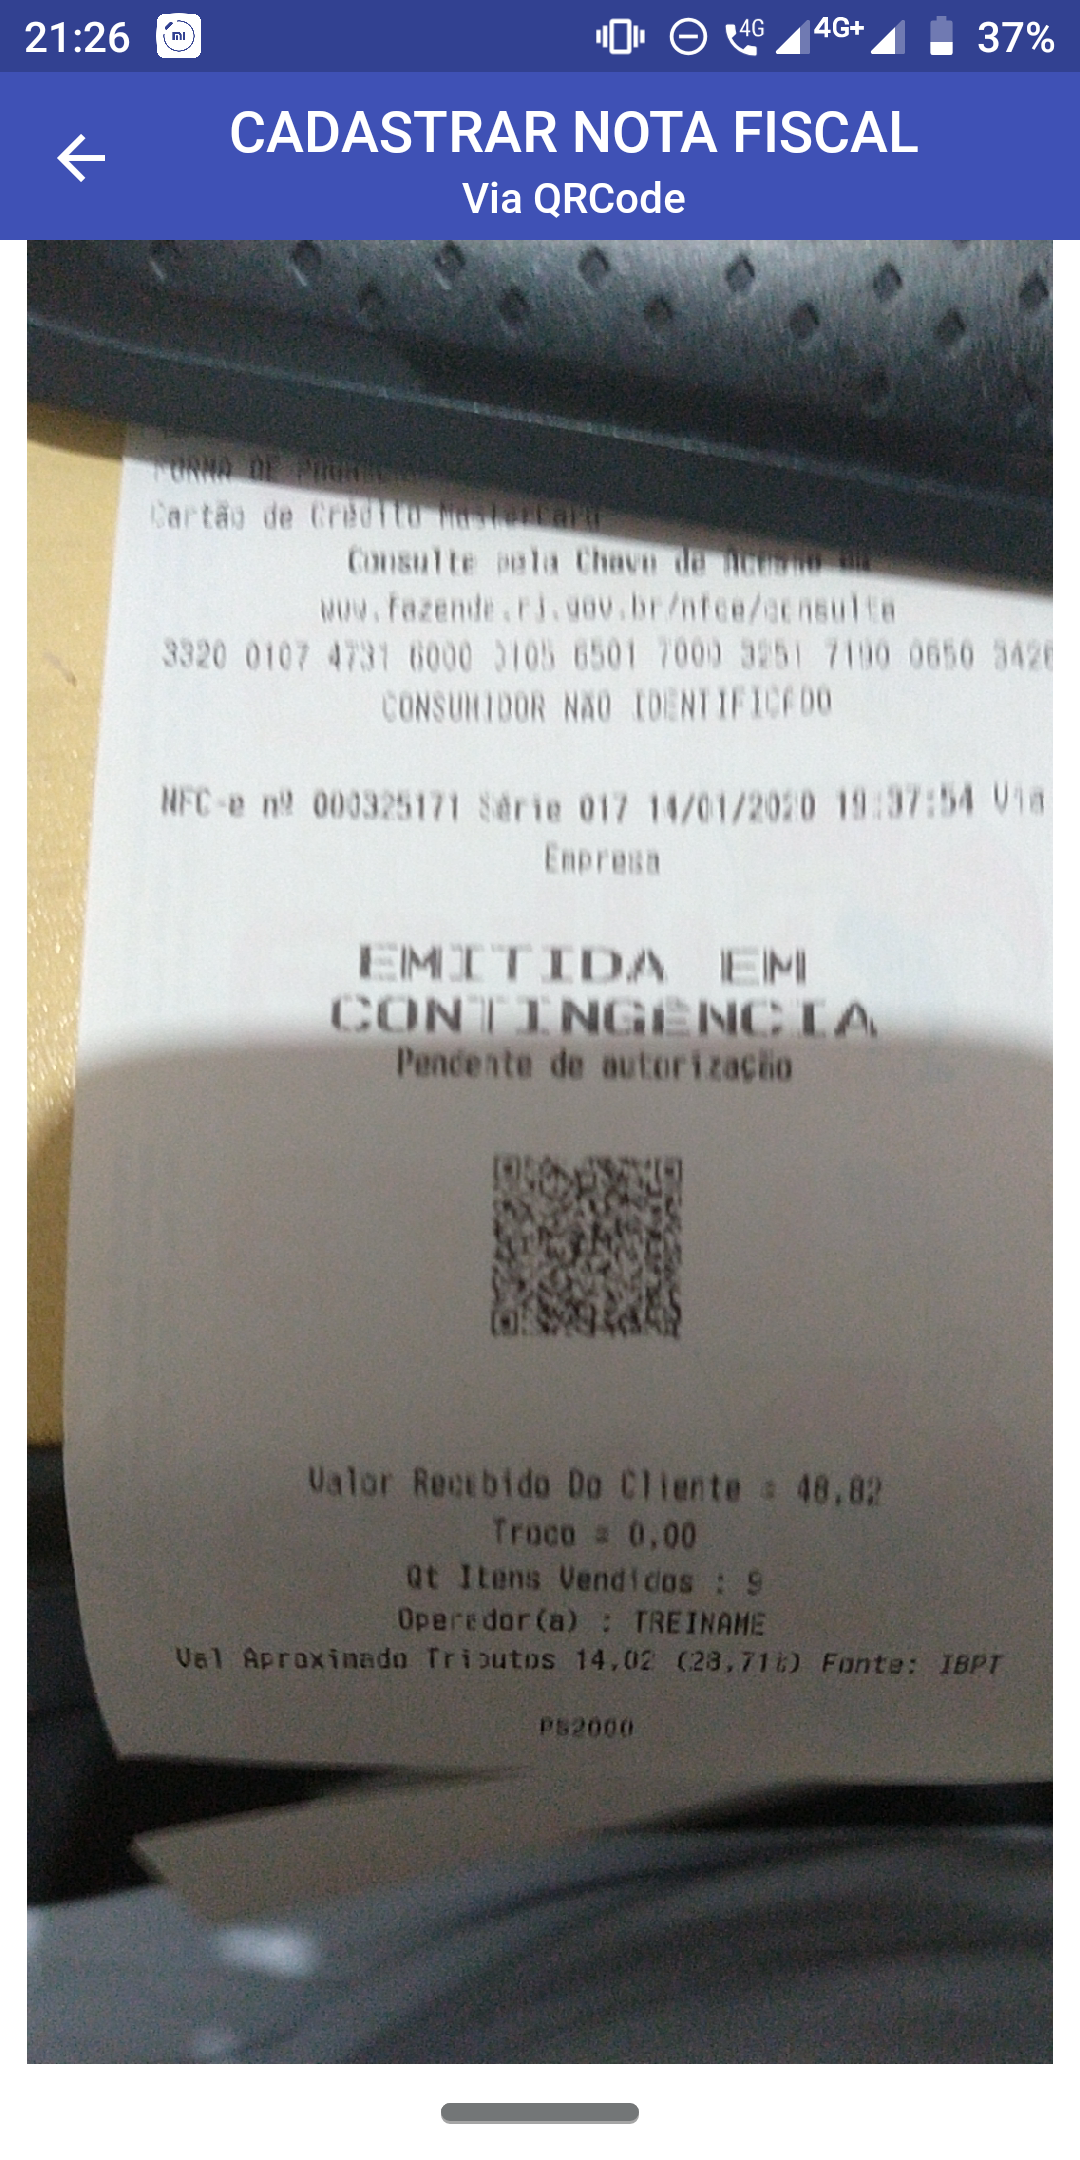
\includegraphics[scale=0.15]{tcc/figures/app/app_qrcode_solicitacao.png}
    \caption{Exemplo de adição de uma NFC-e real via uso do QRCode}
    \label{appQRCodeSolicitacaoFig}
\end{figure}

\subsubsection{Através de Código de Acesso}

\subsection{Busca de Produtos}


\section{Prós e Contras do Desenvolvimento}

% TODO: Falar dos bugs encontrados
% Dificuldades encontradas. Utilizar slide das reuniões.

\section{Limitações do aplicativo e das tecnologias utilizadas}
\subsection{Desvantagens do tipo de Banco de Dados Utilizado}
%Desvantagens da tecnologia utilizada pelo BD:
%Comparar os tipos de BDs: relacionais e não-relacionais;

\section{O Banco de Dados Centralizado}
% Deve ter essa secção?
% Discutir sobre o BD no celular do usuário vs um BD central;
% Já foi falado no Cap3

\section{Trabalhos Futuros}
%Registros do usuário;
%Monitorar para diferentes mercados, produtos e cidades;

% Tratamento no QRCode com problema na leitura. Pós processamento na imagem.

% Falar da tentativa de salvar para leitura posterior.